%%%%%%%%%%%%%%%%%%%%%%%%%%%%%%%%%%%%%%%%%
% Wenneker Article
% LaTeX Template
% Version 2.0 (28/2/17)
%
% This template was downloaded from:
% http://www.LaTeXTemplates.com
%
% Authors:
% Vel (vel@LaTeXTemplates.com)
% Frits Wenneker
%
% License:
% CC BY-NC-SA 3.0 (http://creativecommons.org/licenses/by-nc-sa/3.0/)
%
%%%%%%%%%%%%%%%%%%%%%%%%%%%%%%%%%%%%%%%%%

%----------------------------------------------------------------------------------------
%	PACKAGES AND OTHER DOCUMENT CONFIGURATIONS
%----------------------------------------------------------------------------------------

\documentclass[10pt, a4paper, twocolumn]{article} % 10pt font size (11 and 12 also possible), A4 paper (letterpaper for US letter) and two column layout (remove for one column)

%%%%%%%%%%%%%%%%%%%%%%%%%%%%%%%%%%%%%%%%%
% Wenneker Article
% Structure Specification File
% Version 1.0 (28/2/17)
%
% This file originates from:
% http://www.LaTeXTemplates.com
%
% Authors:
% Frits Wenneker
% Vel (vel@LaTeXTemplates.com)
%
% License:
% CC BY-NC-SA 3.0 (http://creativecommons.org/licenses/by-nc-sa/3.0/)
%
%%%%%%%%%%%%%%%%%%%%%%%%%%%%%%%%%%%%%%%%%

%----------------------------------------------------------------------------------------
%	PACKAGES AND OTHER DOCUMENT CONFIGURATIONS
%----------------------------------------------------------------------------------------

\usepackage[english]{babel} % English language hyphenation

\usepackage{microtype} % Better typography

\usepackage{amsmath,amsfonts,amsthm} % Math packages for equations

\usepackage[svgnames]{xcolor} % Enabling colors by their 'svgnames'

\usepackage[hang, small, labelfont=bf, up, textfont=it]{caption} % Custom captions under/above tables and figures

\usepackage{booktabs} % Horizontal rules in tables

\usepackage{lastpage} % Used to determine the number of pages in the document (for "Page X of Total")

\usepackage{graphicx} % Required for adding images

\usepackage{enumitem} % Required for customising lists
\setlist{noitemsep} % Remove spacing between bullet/numbered list elements

\usepackage{sectsty} % Enables custom section titles
\allsectionsfont{\usefont{OT1}{phv}{b}{n}} % Change the font of all section commands (Helvetica)

 \usepackage{setspace} \doublespacing 
\usepackage[switch]{lineno} 

% \usepackage{amsmath}
% \usepackage{breqn}
\usepackage{mathtools}

%----------------------------------------------------------------------------------------
%	MARGINS AND SPACING
%----------------------------------------------------------------------------------------

\usepackage{geometry} % Required for adjusting page dimensions

\geometry{
	top=1cm, % Top margin
	bottom=1.5cm, % Bottom margin
	left=2cm, % Left margin
	right=2cm, % Right margin
	includehead, % Include space for a header
	includefoot, % Include space for a footer
	%showframe, % Uncomment to show how the type block is set on the page
}

\setlength{\columnsep}{7mm} % Column separation width

%----------------------------------------------------------------------------------------
%	FONTS
%----------------------------------------------------------------------------------------

\usepackage[T1]{fontenc} % Output font encoding for international characters
\usepackage[utf8]{inputenc} % Required for inputting international characters

\usepackage{XCharter} % Use the XCharter font

%----------------------------------------------------------------------------------------
%	HEADERS AND FOOTERS
%----------------------------------------------------------------------------------------

\usepackage{fancyhdr} % Needed to define custom headers/footers
\pagestyle{fancy} % Enables the custom headers/footers

\renewcommand{\headrulewidth}{0.0pt} % No header rule
\renewcommand{\footrulewidth}{0.4pt} % Thin footer rule

\renewcommand{\sectionmark}[1]{\markboth{#1}{}} % Removes the section number from the header when \leftmark is used

%\nouppercase\leftmark % Add this to one of the lines below if you want a section title in the header/footer

% Headers
\lhead{} % Left header
\chead{\textit{\thetitle}} % Center header - currently printing the article title
\rhead{} % Right header

% Footers
\lfoot{} % Left footer
\cfoot{} % Center footer
\rfoot{\footnotesize Page \thepage\ of \pageref{LastPage}} % Right footer, "Page 1 of 2"

\fancypagestyle{firstpage}{ % Page style for the first page with the title
	\fancyhf{}
	\renewcommand{\footrulewidth}{0pt} % Suppress footer rule
}

%----------------------------------------------------------------------------------------
%	TITLE SECTION
%----------------------------------------------------------------------------------------

\newcommand{\authorstyle}[1]{{\large\usefont{OT1}{phv}{b}{n}\color{Black}#1}} % Authors style (Helvetica)

\newcommand{\institution}[1]{{\footnotesize\usefont{OT1}{phv}{m}{sl}\color{Black}#1}} % Institutions style (Helvetica)

\usepackage{titling} % Allows custom title configuration

\newcommand{\HorRule}{\color{Black}\rule{\linewidth}{1pt}} % Defines the gold horizontal rule around the title

\pretitle{
	\vspace{-30pt} % Move the entire title section up
	\HorRule\vspace{10pt} % Horizontal rule before the title
	\fontsize{32}{36}\usefont{OT1}{phv}{b}{n}\selectfont % Helvetica
	\color{Black} % Text colour for the title and author(s)
}

\posttitle{\par\vskip 15pt} % Whitespace under the title

\preauthor{} % Anything that will appear before \author is printed

\postauthor{ % Anything that will appear after \author is printed
	\vspace{10pt} % Space before the rule
	\par\HorRule % Horizontal rule after the title
	\vspace{20pt} % Space after the title section
}

%----------------------------------------------------------------------------------------
%	ABSTRACT
%----------------------------------------------------------------------------------------

\usepackage{lettrine} % Package to accentuate the first letter of the text (lettrine)
\usepackage{fix-cm}	% Fixes the height of the lettrine

\newcommand{\initial}[1]{ % Defines the command and style for the lettrine
	\lettrine[lines=3,findent=4pt,nindent=0pt]{% Lettrine takes up 3 lines, the text to the right of it is indented 4pt and further indenting of lines 2+ is stopped
		\color{DarkGoldenrod}% Lettrine colour
		{#1}% The letter
	}{}%
}

\usepackage{xstring} % Required for string manipulation

\newcommand{\lettrineabstract}[1]{
	\StrLeft{#1}{1}[\firstletter] % Capture the first letter of the abstract for the lettrine
	\initial{\firstletter}\textbf{\StrGobbleLeft{#1}{1}} % Print the abstract with the first letter as a lettrine and the rest in bold
}

%----------------------------------------------------------------------------------------
%	BIBLIOGRAPHY
%----------------------------------------------------------------------------------------
% \usepackage{natbib}
% \bibliographystyle{molecularEcology.bst}

\usepackage[backend=biber,style=apa,natbib=true]{biblatex} % Use the bibtex backend with the authoryear citation style (which resembles APA)

\addbibresource{tellis.bib} % The filename of the bibliography

\usepackage[autostyle=true]{csquotes} % Required to generate language-dependent quotes in the bibliography
 % Specifies the document structure and loads requires packages

%----------------------------------------------------------------------------------------
%	ARTICLE INFORMATION
%----------------------------------------------------------------------------------------

\title{Joint estimation of paternity, sibships and pollen dispersal in a snapdragon hybrid zone} % The article title

\author{
	\authorstyle{
        Thomas James Ellis\textsuperscript{1,2},
        David Luke Field, \textsuperscript{3,4},
        Nicholas H. Barton\textsuperscript{1,*}} % Authors
	\newline\newline % Space before institutions
	\textsuperscript{1}\institution{Institute of Science and Technology Austria, 2234 Klosterneuburg, Austria}\\ % Institution 1
	\textsuperscript{2}\institution{Gregor Mendel Institute of Molecular Plant Sciences, Doktor-Bohr-Gasse 3, 1030 Vienna, Austria}\\ % Institution 2
	\textsuperscript{3}\institution{Applied Biosciences, Macquarie University, Sydney, New South Wales, Australia}\\ % Institution 3
    \textsuperscript{4}\institution{School of Science, Edith Cowan University, Joondalup, Western Australia, Australia}\\ % Institution 4
    \textsuperscript{*}\institution{To whom correspondence should be addressed: nick.barton@ist.ac.at} 
}

% Example of a one line author/institution relationship
%\author{\newauthor{John Marston} \newinstitution{Universidad Nacional Autónoma de México, Mexico City, Mexico}}

\date{\today} % Add a date here if you would like one to appear underneath the title block, use \today for the current date, leave empty for no date

%----------------------------------------------------------------------------------------

\begin{document}

\maketitle % Print the title

\thispagestyle{firstpage} % Apply the page style for the first page (no headers and footers)
\linenumbers
%----------------------------------------------------------------------------------------
%	ABSTRACT
%----------------------------------------------------------------------------------------

% \lettrineabstract{}

\section{Abstract}
The distribution of pollen dispersal distances sets the scale for plant population dynamics.
A useful approach for inferring the distribution dispersal distances is to infer the distances between mates by paternity or parentage reconstruction.
This is most powerful when information about multiple properties or data types are inferred in a joint analysis.
We describe an approach to jointly infer paternity, sibling relationships and population parameters, with the example of the pollen dispersal kernel in a natural population of the yellow-flowered \textit{Antirrhinum majus striatum} and the magenta-flowered \textit{A. m. pseudomajus}.
Pollen dispersal is leptokurtic, with half of mating events occurring within 30m, but with a long tail of mating events up to 747m.
We also find tentative evidence that fathers tend to be to the East of mothers, indicating that there is a bias in pollen dispersal from \textit{A. m. pseudomajus} into \textit{A. m. striatum}.
The scale of pollen dispersal is large enough that pollinators should encounter the full range of hybrid phenotypes in the hybrid zone, and would be sufficient for any pollinator-mediated selection to influence male or female fitness.

%----------------------------------------------------------------------------------------
%	ARTICLE CONTENTS
%----------------------------------------------------------------------------------------

\section{Introduction}

Knowledge of the genealogical relationships between individuals - their pedigree - is an extremely useful tool for understanding natural populations because it gives a direct estimate of who mates with whom, and differences in reproductive success \citep{thompson1976inference, pemberton2008wild}.
One example, pedigrees can tell us about the distribution of dispersal distances organisms or gametes travel during their lifetimes, which sets the scale at which populations vary (\cite{cain2000long, kremer2012long}).
Of particular interest is both the average distance travelled and the shape of the dispersal distribution \citep{cain2000long, nathan2012dispersal}.
In plants, dispersal is often characterised by leptokurtic or 'fat-tailed' distributions, where dispersal is most likely to occur over short distances, but there is a long tail of long-range dispersal events (\cite{clark1998trees,austerlitz2004using,bullock2017synthesis}).
This leptokurtosis allows much more rapid dispersal than would be suggested by the average dispersal distance alone, with long-range migrants having a disproportionate effect on the spread of adaptive alleles (\cite{clark1998trees,cain2000long}).
We thus aim to reconstruct mating events between individuals to infer the distribution of dispersal.

Pedigrees are inferred using three sources of information.
First, the oldest and most common approach is to identify parent-offspring relationships that are most likely given on Mendelian inheritance, treating offspring individuals separately \citep{thompson1976inference, meagher1986analysis, marshall1998statistical}.
Second, sibling-reconstruction approaches use information about alleles shared between siblings to jointly infer sibling relationships with the parentage of the entire sibship (e.g. \cite{thompson1987parental, emery2001assignment, thomas2002sibship, jones2007estimating, wang2004sibship, anderson2016bayesian, huisman2017pedigree}).
Because sibling relationships are typically not known and there are a very large number of possible configurations to consider, a major challenge in sibship inference is to explore this space effectively.
Genetic information shared between parents, offspring and between siblings are vital for reconstructing their relationships.

Finally, mating patterns and differences in mating success often depend on additional population and phenotypic factors that are not related to genetics.
Jointly modelling these processes with pedigree relationships can not only better resolve relationships between individuals, but is also often of direct interest itself \citep{neff2001bayesian, hadfield2006towards}.
Pollen dispersal is a good example of this.
We expect nearby individuals to mate with one another more than with more distant individuals.
By using as suitable model for how the probability of mating decays with distance we expect to weight inference to more likely candidate mates, but also to directly infer meaningful parameters about pollen flow \citep{adams1992using, jones2003maximum, oddou2005pollen, klein2008pollen, chybicki2013seeing}.
A particularly well-established approach for this the the 'neighbourhood model' which jointly estimates parent-offspring relationships and dispersal distributions whilst also accounting for pollen immigration, incomplete sampling, variation in fertility and assortative mating \citep{adams1989mating, burczyk2004cautions, oddou2005pollen, chybicki2013seeing, gerard2006assortative, chybicki2018nmpi, chybicki2021identification}.
Jointly modelling parent-offspring relationships with population parameters has great appeal because it allows us to directly address biologically relevant relationships between traits of interest and mating patterns.

Augmenting parentage information with information about sibling relationships or population parameters is expected to increase the accuracy of pedigree reconstruction \citep{neff2001bayesian, wang2007parentage}.
However, we currently lack a framework for utilising all three sources of information - parentage, sibships and population parameters - in a single joint analysis.
Because of this, we also lack an understanding of the relative contribution of sibship and population parameters to pedigree inference, and how this changes depending on the data available and the biology of the system.
We previously described a package Fractional Analysis of Paternity and Sibships (FAPS) to jointly infer of paternity and sibships (\cite{ellis2018efficient}).
In this paper we describe how to include non-genetic information into the FAPS procedure, and use MCMC to update parameters for those data to jointly infer paternity, sibships and population parameters.
We then apply this to the inference of the pollen dispersal distribution in a hybrid-zone population of the snapdragon \textit{Antirrhinum majus} with a large number of potential pollen donors.
Using simulations we also characterise how the power to reconstruct paternity of individuals and mating between adults depends on the information available from genetics markers, the degree of shared paternity and the scale of pollen dispersal.

%------------------------------------------------

\section{Materials and Methods}

\subsection{\textit{A. majus} data}

\subsubsection{Study population}

\begin{figure*}
    \centering
	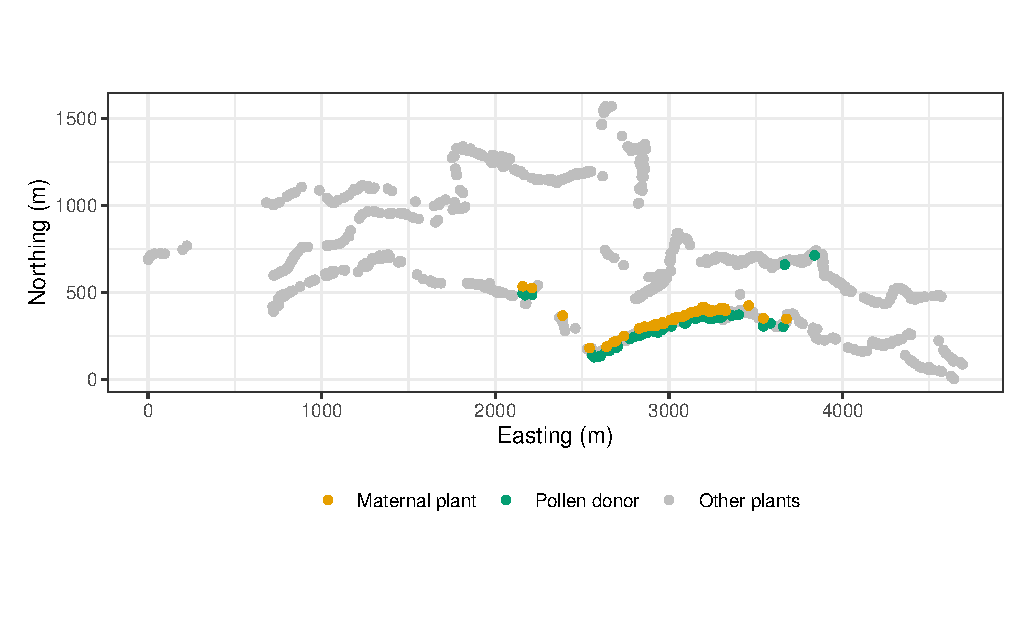
\includegraphics[]{fig-map.eps} % Figure image
	\caption{
        Map of the hybrid zone.
        The map shows the distribution of maternal plants, inferred pollen donors and remaining plants along the lower (South) and upper (North) roads. Only pollen donors for families with one or more offspring are shown.}
	\label{fig:map} % Label for referencing with \ref{bear}
\end{figure*}

We examine a hybrid zone population of the snapdragon \textit{Antirrhinum majus} in the Spanish Pyrenees. Here, the yellow-flowered \textit{A. m. striatum} and the magenta-flowered \textit{A. m. pseudomajus} meet and hybridise to produce diverse recombinant phenotypes, including pink, white and orange flowers.
The population grows along two parallel roads running East-West close to Rib\`{e}s de Freser (figure \ref{fig:map}). The ’lower’ road is at 1150-1200m above sea level, whilst the ’upper’ road climbs 1250-1500m, and is 500-1000m north of the lower road. Hybrids are mostly confined to a 1km ’core’ hybrid zone, with \textit{A. m. striatum}- and \textit{A. m. pseudomajus}-like plants becoming dominant to the West and East respectively. We surveyed as many flowering plants as we could find in June and July of 2012 (n=2124), and collected information on flower number and location using a Trimble GeoXT datalogger. We collected two to three leaves for DNA extraction and dried these in silica gel (Fischer Scientific). \textit{A. majus} grows in disturbed habitats such as roadsides and railways; they are rare in the established forest and pasture between the two roads, on the north-facing slope to the South, and on the high mountain peak to the North of the two roads (figure \ref{fig:map}. It thus is likely that we sampled the majority of the plants that flowered during the study period, although we cannot exclude that some flowering may have occurred before or after this. 

Pollination is carried out exclusively by large bumblebees and carpenter bees who are large enough to open the flowers (\cite{vargas2010occluded, andalo2019prevalence}). \textit{A. majus} has a gametophytic self-incompatibility system, and self-pollinated seeds are very rare \parencite{surendranadh2022effects}. There are no detectable post-zygotic barriers between \textit{A. m. striatum} and \textit{A. m. pseudomajus} (\cite{andalo2010post}).

In August 2012 we collected a single, mature, wild-pollinated fruit from each of 60 mothers (figure \ref{fig:map}). In order to minimise disturbance to the population we only sampled from plants which had set a minimum of five mature fruits. These mothers were chosen to represent an even sample of pigmentation genotypes, spread as evenly as possible across the core of the hybrid zone where hybrids are most dense, resulting in 10 \textit{A. m. striatum}-like, 17 \textit{A. m. pseudomajus}-like, and 33 hybrid-phenotype mothers.

\subsubsection{Genotyping}

We grew seeds in 5cm plug trays filled with potting compost (Gramaflor) in a greenhouse under Sylvania GroLux lights on a 16-hour cycle. We sowed three seeds per plug for 50-70 plugs per maternal family and thinned seedlings to a single seedling per plug after cotelydons had appeared. We transferred approximately 1cm$^2$ of fresh tissue from 1419 seedlings to 96-well DNA-extraction plates (LGC Genomics, Berlin) and allowed tissue to dry using the sample bag and silica gel provided. For parental tissue from the hybrid zone we transferred approximately 1cm$^2$ tissue dried in the field to the same plates. DNA extractions of the plated tissue samples were carried out by LGC Genomics.

We genotyped tissue samples at 71 SNPs by KASPR sequencing (LGC Genomics).
These SNPs are a subsample of a panel used for a wider survey of the hybrid zone (\cite{surendranadh2022effects}).
Previous work identified the per-locus genotyping error rate in these data to be approximately $10^4$ (\cite{surendranadh2022effects}).
We removed 110 offspring that had missing data at more than 20\% of the SNPs.
We also pruned 4 SNPs that showed more than 20\% missing data, or less than 15\% heterozygosity.
This left us with a set of 1308 offspring from 60 maternal families and 2124 candidate pollen donors, with between three and 39 offspring per maternal family (mean=21.8), with 64 marker SNPs.

\subsection{Joint estimation of paternity, sibships and dispersal}

\subsubsection{Probability model}

We begin with observed SNP marker data \textbf{M} for mothers, offspring and candidate father, and a matrix \textbf{D} of Euclidean distances between mothers and all possible candidate fathers, and the per-locus genotyping error rate $\epsilon$. From this we wish to infer pedigree P describing sibling, paternal and (known) maternal relationships, and vector $\theta$ of dispersal parameters. The full probability model is then
\begin{equation}
\label{eqn:probability_model}
\begin{split}
\Pr( P, \theta | \textbf{M}, \textbf{D}, \epsilon) \propto \Pr(\textbf{M} | P, \textbf{D}, \theta, \epsilon)
\Pr(\textbf{D} | \theta, P) \\
\Pr(\theta) \Pr(P) \Pr(\epsilon)
\end{split}
\end{equation}

In the following sections we outline how to extend our existing method for inferring sibships and paternity to include data from non-genetic covariates, a model for pollen dispersal, suitable hyperprior distributions for dispersal parameters, and a procedure to infer the posterior distribution of the parameters of interest.

\subsubsection{Allowing for covariates in paternity inference}

We have previously described a Python package FAPS which performs joint analysis of paternity and sibship relationships for sibling arrays based on SNP data, and allows for integrating out uncertainty in relationships (\cite{ellis2018efficient}). Here we extended the software to allow for additional non-genetic information to be included.

FAPS begins with marker data for one or more maternal families composed of a mixture of half- and full-siblings, the known mother of each family, and an array of candidate fathers.
\textcite{ellis2018efficient} described a method to infer sibling and paternity relationships in those individuals; we refer the reader to that paper for the full details, but review the most important aspects here.
FAPS uses marker data \textbf{M} to build matrix \textbf{G} of probabilities of paternity based on Mendelian transition probabilities for each maternal family.
\textbf{G} has a row for each offspring and a column for each candidate father, where element $g_{ij}$ is the probability that candidate \textit{j} is the father of offspring \textit{i} given marker data, and an estimate of genotyping error rate $\epsilon$. 
The final column of \textbf{G} is the probability that the father of each offspring was missing from the sample of candidates, based on the probability of observing offspring alleles from population allele frequencies.
Rows in \textbf{G} sum to one, and describe a multinomial distribution of probabilities of paternity over all candidate fathers. FAPS then builds a similarity matrix whose \textit{ih}\textsuperscript{th} element is the likelihood

\begin{equation}\label{eqn:faps_similarity_matrix}
    \Sigma_j^F g_{ij}g_{hj}
\end{equation}

that the \textit{i}\textsuperscript{th} and \textit{h}\textsuperscript{th} offspring are full siblings by summing over the probabilities that they share any one of the $F$ fathers. The similarity matrix is used to perform hierarchical clustering to identify plausible ways to partition offspring into families of possible full sibships, and the likelihood of each partition structure is estimated by Monte-Carlo simulation. The likelihood that candidate father \textit{j} is the father of putative full sibship \textit{k} is then
\begin{equation}\label{eqn:faps_lik_sibship}
\Pi_i^n g_{ij}
\end{equation}
for all \textit{n} offspring in \textit{k}. FAPS returns a vector of probabilities (which sum to one) that each candidate is the father of sibship \textit{k}, or that the true father was not sampled. This is done for each plausible partition structure. This gives a distribution of possible partition structures and their likelihoods, and a distribution of paternity probabilities for each putative family within each partition structure.

We can incorporate non-genetic information about paternity using a suitable function relating those data into probabilities of paternity.
In principle this can be done for any kind of data for which there is a suitable function relating the observed data for a set of candidate fathers to a probability of having mating with each mother, given a set of parameter values for that function. The goal is to find parameter values that best explain the data. For example, a standardised continuous phenotype $z$ could be modelled with the logistic function $1/(1+e^{\beta z})$, where $\beta$ describes the relationship between $z$ and male fertility.
A categorical phenotype can be modelled as a multinomial vector of probabilities that sum to one.
In this study we use matrix \textbf{D} of Euclidean distances between mothers and candidate fathers as a covariate, and model the probability $\Pr(d_{mj}|\theta)$ of a mating event occurring between mother \textit{m} and candidate \textit{j} who are distance $d_{mj}$ apart, based on a suitable model of pollen dispersal (see below).
It is then straightforward to incorporate this into the procedure outlined above by modifying eqn. \ref{eqn:faps_similarity_matrix} to
\begin{equation}\label{eqn:pairwise_with_covariates}
\Sigma_j^F \Pr(d_{mj} | \theta)g_{ij}g_{hj}
\end{equation}
and eqn. \ref{eqn:faps_lik_sibship} to
\begin{equation}
\label{sibship_with_covariates}
\Pr(d_{mj} | \theta)\Pi_i^n g_{ij}
\end{equation}

Eqn. \ref{sibship_with_covariates} can then be used to estimate the likelihood of the partition structure by Monte-Carlo simulation, as previously described by \textcite{ellis2018efficient}.
For a given set of dispersal parameters in $\theta$ the likelihood of the whole maternal family is then the sum of likelihoods for each possible partition. When there are multiple maternal families, the likelihood of the whole dataset given $\theta$ is the product of those likelihoods over each maternal family. When we update $\theta$, this likelihood will change, giving us a way to compare likelihoods of different dispersal parameter values and identify those most consistent with the data.

A special case arises when it is known that offspring are unrelated, or that sibship structure is otherwise known. In this case the likelihood of the data can be calculated by summing the likelihoods of paternity for each candidate father on the $k^{th}$ full-sibship, and multiplying over all $K$ full sibships:
\begin{equation}
    \label{eqn:lik_if_no_structure}
    \Pi_k^K\Sigma_j^F\Pr(d_{mj} | \theta)\Pi_i^n g_{ij}
\end{equation}
This obviates the need for likelihood estimation by Monte-Carlo simulation.

\subsubsection{Pollen dispersal distribution}

We wish to describe the distribution of distances travelled by pollen from anther to stigma \citep{nathan2012dispersal}.
A useful function for describing plant dispersal distributions is the generalised normal distribution (\cite{clark1998trees,Nadarajah2005,kremer2012long}). This is a generalisation of the exponential family of probability distributions and includes the exponential and standard normal distributions as special cases, but allows for fat and thin tails. It is commonly used to model plant dispersal distributions because these are often found to show clear kurtotis (e.g. \cite{austerlitz2004using, robledo2005patterns, klein2008pollen, burczyk2019patterns, field2011importance, ottewell2012pollen}). The generalised normal distribution describes the probability of observing dispersal distance \textit{d} given scale parameter $a$ and shape parameter $b$:
\begin{equation}
\Pr(d|a,b) = \exp{  (-|\frac{d}{a}| ^b) }
\label{eqn:GND}
\end{equation}
The function takes the forms of the standard exponential when $b=1$ and normal distribution when $b=2$. Values of $b<1$ reflect leptokurtic distributions with tails that decay more slowly than would be expected under the exponential distribution. Using $\theta={a,b}$, this provides a convenient function for calculating $\Pr(d_{mj} | \theta)$ because it allows for a long tail of long-distance migrants.

Sometimes it may be that an unrelated candidate has a similar or higher probability of paternity of one or more offspring simply due to stochasticity in Mendelian sampling.
Whereas true fathers are expected to be (on average) close to the mother, other candidates should be drawn at random from the population. This will inflate the apparent kurtosis in the data and bias $b$ downwards.
To accommodate this we modify \ref{eqn:GND} to model dispersal as a mixture of a generalised-normal and a uniform distribution:
\begin{equation}\label{eqn:mixture_model}
\Pr(d_{mj} | a,b,\lambda) = \lambda K e^{  (-\frac{d}{a} )^b } + \frac{1-\lambda}{F}
\end{equation}
where $F$ is the number of candidate fathers and $\lambda$ is a mixture parameter determining the proportion of the probability mass due to ’real’ dispersal.
The uniform part of this mixture allows for signal coming from incorrect candidates without requiring the 'true' dispersal kernel to be unnecessarily leptokurtotic.
$\lambda$ also provides an approximate estimate for what the rate of false-postive assignment to medium- and long-distance candidates would have been if this had been ignored.

It is common to also report the mean dispersal distance as the square root of the variance of this distribution as
\begin{equation}
\label{eqn:sd_GND}    
\sqrt{ \frac{ a^2 \Gamma(3/b) }{ \Gamma(1/b) } }
\end{equation}
(\cite{Nadarajah2005}).
We prefer to focus on median dispersal distances because this is more intuitive for highly skewed distributions, and also to estimate this on realised inter-mate distances rather than on parameters alone (see "Inference of mating patterns"). We nevertheless report this and how it relates to the effect of $\lambda$ on results.

\subsubsection{Priors for dispersal parameters}

We require prior distributions for dispersal parameters $a$, $b$ and $\lambda$.

We used a log-normal prior for $b$ ($\ln b \sim N(\mu=0, \sigma = 0.5)$.
This model allows for a range of shape values reflecting leptokurtosis to Gaussian dispersal, but is skeptical about very strong over- or under-dispersion in the dispersal distribution because prior probabilties approach zero as $b$ approaches 0 or 3 (figure S1).
We used a Gamma prior for $a$ because this describes positive continuous values, and because it is conjugate with the variance parameter of a Gaussian distribution.
Because the effect of $a$ depends on $b$ and has no intuitive biological interpretation itself, we used prior simulations to choose a suitable parameterisation for $a$. We first simulated 10000 pairs of values for $a$ and $b$ from Gamma and log-normal distributions respectively. We then used each pair of simulated values to parameterise a generalised normal distribution, and simulated 1000 dispersal distances from that distribution, and visually examined the distribution for biological plausibility. We chose a Gamma distribution with shape=6 and scale=50, because this gave dispersal distributions with most dispersal occurring within 500m, but allowing for rare long-range dispersal events (figure S1).

For $\lambda$, we use a beta distribution with parameters Beta(1.1, 1.1).
This distribution approaches zero when $\lambda$ is close to zero or one, but is fairly flat in between.
This implies that we do not expect that all the weight should be on either the generalised-normal or the uniform components of the mixture distribution in eqn. \ref{eqn:mixture_model}, but that we do not have strong prior beliefs about values between that.
To examine the effect of modelling dispersal as a mixture model at all, we also repeated the MCMC with with $\lambda$ to set to one.

\subsection{Inference}

\subsubsection{Inference via MCMC}

We used the Metropolis-Hastings Markov-chain Monte Carlo algorithm to infer the posterior distribution of dispersal parameters $a$, $b$ and $\lambda$.
We ran four independent chains beginning from distant areas of the parameter space.
At each iteration, we perturbed the value of each parameter by a factor drawn from a normal distribution with a fixed standard deviation for each parameter ($\sigma= 2$ for $a$; $\sigma= 0.05$ for $b$; $\sigma= 0.025$ for $\lambda$).
We ran each chain for 3000 iterations and subsequently removed the first 500 iterations of each as burn-in.
After checking chain convergence we thinned subsequent iterations to retain 250 posterior draws from each chain for further analyses, for a total of 1000 posterior draws.

\subsubsection{Inference of mating events}

We aimed to create a list of possible mating events between mothers and candidate fathers consistent with the data to identify a set of independent pollen dispersal events.
FAPS generates one or more partition structures that a half-sibling family could be split into full-sibling families.
For each partition structure, FAPS identifies valid set of distinct fathers for each full sibship, and estimates a likelihood for each father-sibship configuration.
Each set of fathers reflects a hypothetical set of mating events, and the probability that a single father mated with the maternal plant is the sum of probabilities for each partition structure in which he sires at least one offspring.
This gives a list of mating events, with a posterior probability that each occurred, including an entry for offspring whose father was missing.
The posterior estimate of offspring number is the number of offspring for each father in each father-sibship configuration weighted by the probability of the mating event.
Note that the number and size of sibships are not necessarily integers because estimates are weighted averages over plausible sibship partition structures.
In particular, hypothetical families can have posterior sizes less than one if the nominal number of offspring is one, but the posterior probability for the family is less than one.

We inferred mating events in this way using eqn. \ref{eqn:faps_lik_sibship} based on dispersal parameter estimates from each of 1000 iterations of the MCMC output.
We also calculated the total number of mating events as the sum of probabilities for all mating events with sampled fathers.
Likewise, we estimated of the number of missing fathers is the sum of probabilities for all mating events for unsampled fathers.
However, FAPS does not distinguish paternal families within groups of offspring of an unsampled father, so this value is a lower bound on the number of unsampled fathers.

Finally, we estimated the relationship between the number of offspring in a maternal array and the number of paternal families therein.
We first averaged paternal family size for each mother-father pair over iterations of the MCMC, then fitted a Poisson generalised linear model (GLM) of paternal family size on maternal family size (\cite{McCullagh1989}).

% \subsubsection{Asymmetric dispersal}

% To test for potential bias in the direction of pollen dispersal we calculated the mean difference in East-West position between mothers and fathers.
% We compared the average asymmetry in direction for observed mating events to simulated mating events as described above.
% Because all but one observed pollen donor turned out to be on the lower road we restricted this analysis to simulated pollen donors on the lower road.

\subsection{Simulations}

We used simulations to determine the statistical power of the dataset and and how this depends on the information used.

We simulated mating events between each true mother and one or more sires drawn from the pool of 2124 genotyped adult plants.
Each maternal plant mated with the same number of pollen donors as inferred in the empirical analysis to generate one or more full-sib families per mother.
For simplicity we drew sires for each family based on the probability of mating with a mother given an exponential pollen dispersal distribution (i.e. $b=1$ and different values for $a$; see below).
We ignored mating events with posterior probabilities less than 0.9.
We simulated offspring genotypes based on Mendelian segregation and added genotyping errors to adults and offspring genotypes with the observed genotype error rate of $10^{-4}$ per locus per individual.
In this way simulated data reflects the the observed genetic and spatial structure of the \textit{A.~majus} hybrid zone.

We parameterised simulations by varying four parameters that are likely to affect inference of relationships.
We aimed to use values that are likely to affect cases where parameters are less informative, moderately informative, and more informative.
To vary marker information we downsampled the number of genotyped markers to 40, 50 and 60.
To vary the information about paternity shared between full siblings we varied he number of offspring sired by each father (1, 3 and 5 offspring)
To simulate missing fathers we randomly selected 10\%, 30\% and 50\% of true sires and removed them from the set of candidate fathers.
We simulated dispersal with mean distances of 3m, 30m and 300m.
We repeated each parameter combination 100 times.

We were interested in two measures of relationship inference.
First, we used FAPS to calculate the accuracy of paternity of individuals, accounting for uncertainty in sibships \cite{ellis2018efficient}.
We generated a table giving the most likely father of each offspring, which may be one of the genotyped candidate fathers or an unsampled 'missing' father, along with the posterior probability for that assignment, and compared this to the known list of fathers.
We calculated the true positive rate as the probability that the the most-probable father is the correct father, among those offspring whose most likely father was not 'missing'.
We calculated a false-negative rate as the probability that the most-probable father was assigned as 'missing' when he was in fact present, among those offspring whose most likely father was missing.
False positive and false negative rates are given by one minus these values respectively.

Second, we inferred plausible mating events accounting for uncertainty in sibship structure as described above.
We previously noted that when FAPS errs, it tends to split one individual in a sibship into a singleton family, but essentially never incorrectly merges unrelated sibships \cite{ellis2018efficient}.
These singleton families will tend to have posterior probabilities of less than one.
This predicts that mating events with family sizes (weighted by posterior probability) less than one are likely to be spurious.
To test this, we calculated the true-positive probability that mating events with weighted family sizes of one or more are correct.
We also calculate the false-negative probability that weighted family sizes of less than one are correct.
This analysis assesses the extent to which focussing on mating events with weighted family sizes  a convenient heuristic for identifying true mating events in empirical data.

Finally, we investigated the contribution of different sources of information to genealogical inference.
For each replicate dataset and parameter combination we calculated the accuracy of paternity and mating-event inference described above in three ways.
We compared results obtained  (1) using only information from paternity (i.e. mother-father-offspring trios), (2) using information from paternity and sibling relationships (as described by \cite{ellis2018efficient}), and (3) using information from paternity, sibships and dispersal distances together (this paper).
This analysis compares the contribution of information from paternity, sibling relationships and mating parameters to the paternity and mating event inference.

\section{Results}

% \subsection{True sibships can be identified with high confidence}

% \begin{figure*}
%     \centering
%     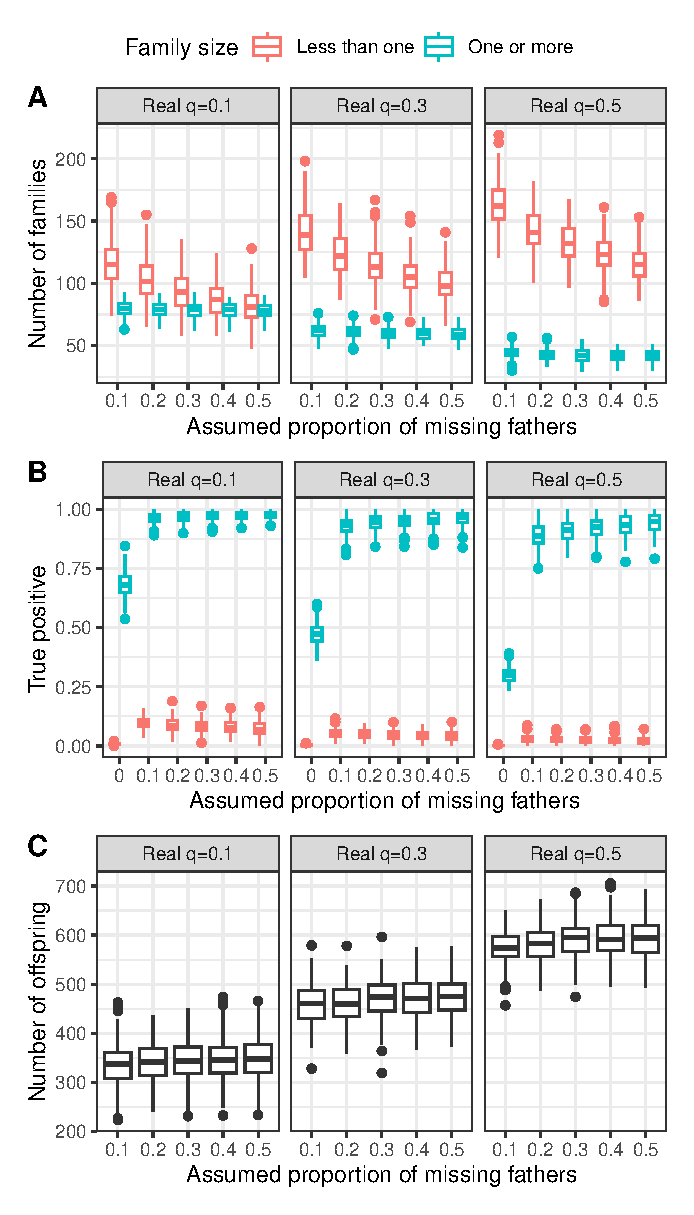
\includegraphics{simulations.eps}
%     \caption{
%         Simulation results.
%         Panels show the true proportion, $q$, of missing fathers; \textit{x}-axes show the assumed proportion used to infer families.
%         (A) Number of paternal families identified with weighted-mean offspring number averaged over plausible sibships greater or less than one.
%         (B) Probability that paternal families identified by FAPS are real.
%         (C) Number of offspring inferred to have an unsampled father.
%     }
%     \label{fig:simulations}
% \end{figure*}

% We found that paternal families inferred from simulated data could be divided into those with family sizes of one or more, and a second group with weighted-mean family sizes less than one (figure \ref{fig:simulations}A).
% Consistent with this, families with one or more offspring overwhelmingly reflect true mating events, whereas those with less than one offspring were overwhelmingly incorrect (figure \ref{fig:simulations}B).
% This indicates that we can reliably identify true mating events by discarding paternal families with weighted-mean family sizes less than one.

% We found surprisingly little effect of prior beliefs about the proportion of missing fathers on the accuracy of paternity inference.
% Focussing on robust paternal families with one or more offspring, the number of families detected decreased as the true number of missing fathers increased, as one would expect (figure \ref{fig:simulations}A).
% However, there was negligible relationship between the number of these families found and the prior expectation about the proportion of missing fathers, even when this prior substantially over- or under-estimated the true value.
% We did find a slight increase in the probability that these inferred mating events were correct with higher input values of $q$ (figure \ref{fig:simulations}B), presumably because increasing the prior probability that a father is unsampled decreases the probability of paternity for candidates who are not true fathers.
% Likewise, the number of offspring assigned to missing fathers increased with the true proportion of missing fathers, but there was no effect of changing the value of proportion of missing fathers used in the analysis (figure \ref{fig:simulations}C).
% These results demonstrate that the prior expectations about the proportion of missing fathers has very little effect on downstream analyses.

% We also note that the observed number of offspring with an unsampled father in the simulations is substantially higher than would be expected from the true proportion of fathers.
% This is because the simulations use the true spatial distribution of maternal and candidate plants, and the same candidate can sire offspring with multiple mothers.
% If that candidate is unsampled, this affects multiple full-sib families.
% As such, assuming our simulation regime is sufficiently realistic, we should expect the proportion of offspring with an unsampled father in the empirical dataset to be higher than the true proportion of missing fathers.

\subsection{Family sizes vary in *A.~majus*}

We identified an average of 195 full-sibling families for which a father could be positively identified across MCMC samples (96\% credible intervals (CI): 189, 199).
6.5\% families had posterior probabilities and posterior-mean family sizes less than one, showed substantial uncertainty across MCMC iterations (figures S2) and seem to be drawn at random from across the population (figure S3), indicating that these mating events are likely to be dubious.
In contrast, the remaining 168 families showed strong posterior support with little variation between MCMC iterations (figure S2), and were clustered closer to the maternal plants (figure S3).
These likely reflect robust independent mating events that can be used to infer a dispersal kernel, and we focus on these mating events in the rest of this manuscript.

Full-sibship sizes ranged from one to 18 (figure S4).
The GLM of the number of full sibships on maternal-family size revealed that (natural) log number of sibships increased by 0.045 for every additional offspring included in the maternal family (intercept~=~0.40; figure S5). This corresponds to detecting a new family for approximately every 4 or 5 offspring genotyped, on average.

For all sixty mothers we found a mating event with non-zero probability for which the father one or more offspring was not sampled (figure S2).
These families include an average of 789 offspring (CIs: 785, 793).
This corresponds to around 60\% of the offspring.

\subsection{Pollen dispersal is leptokurtic and asymmetric}

\begin{figure*}
    \centering
    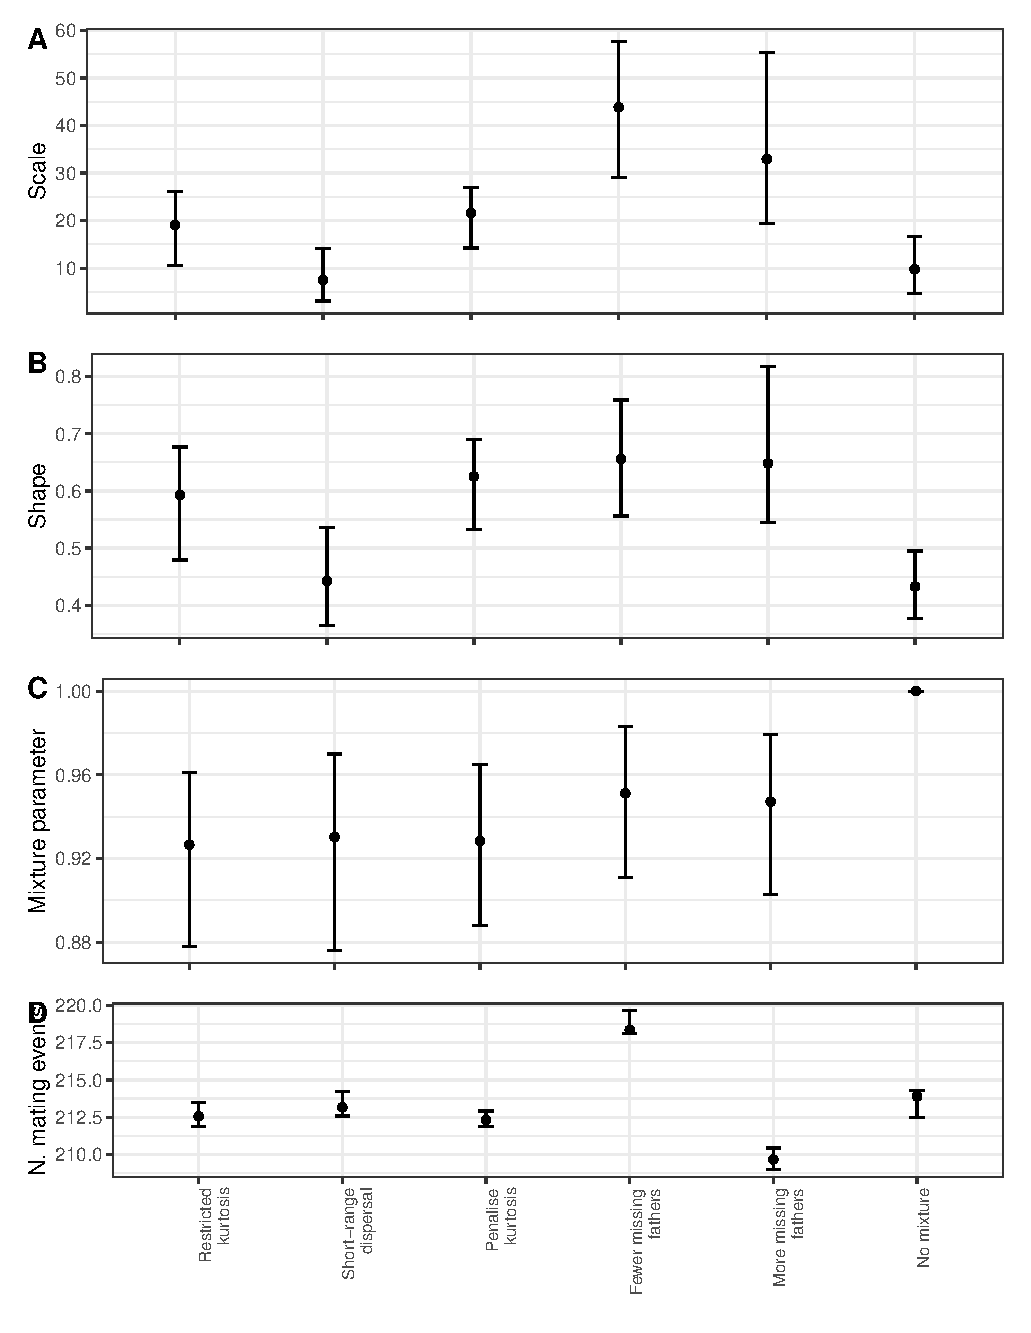
\includegraphics{posterior_distributions.eps}
    \caption{
        Posterior densities for the shape, scale, and mixture parameters of the dispersal kernel.
        Histograms show stacked densities for each of four independent chains.
    }
    \label{fig:posterior_summaries}
\end{figure*}

\begin{figure*}
    \centering
    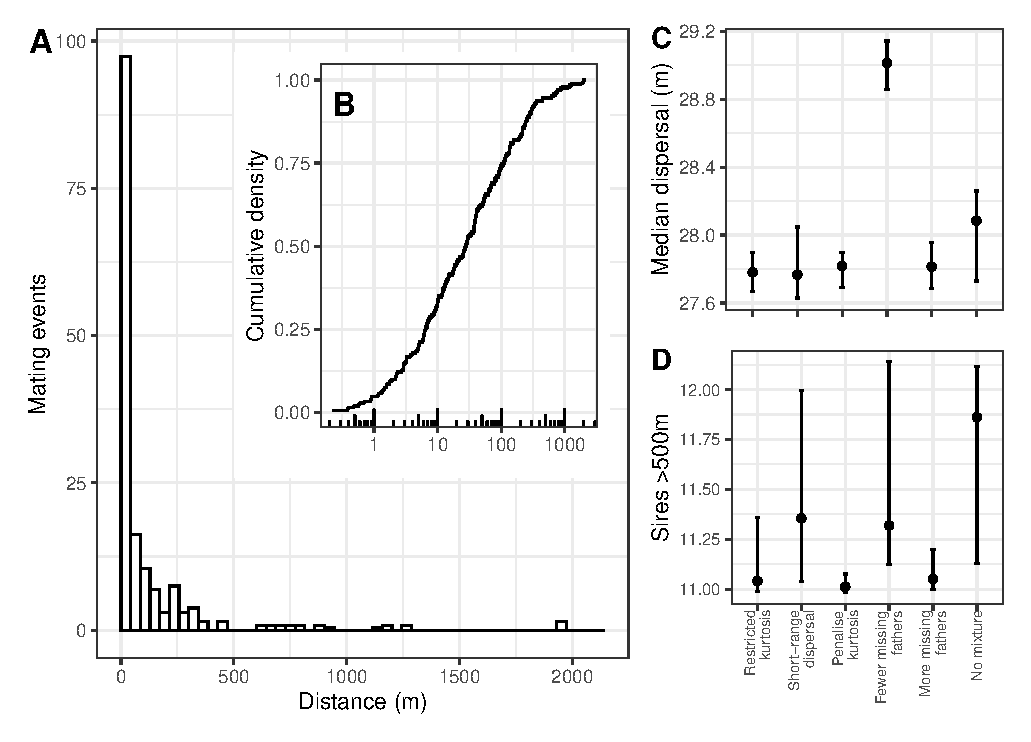
\includegraphics{dispersal.eps}
    \caption{
        Distribution of pollen-dispersal distances.
        (A) Histogram and (B) cumulative distribution of distances for dispersal events for paternal families with one or more offspring.
        Note the log10 scale of the x-axis in B.
        Mating events are weight weighted by their posterior probability.
        The histogram is summed over iterations of the MCMC.
        Separate cumulative curves are shown for 1000 MCMC iterations separately.
    }
    \label{fig:dispersal}
\end{figure*}

The posterior distribution for the dispersal shape parameter was consistently less than one, with a posterior mean of 0.57 (96\% CIs: 0.46, 0.70), indicating a leptokurtic dispersal kernel (figure \ref{fig:posterior_summaries}A).
Posterior mean scale was 22.0 (95\% CIs: 9.1, 37.4; \ref{fig:posterior_summaries}B).
Consistent with this, the distribution of pollen dispersal distances for families with one or more offspring shows a peak close to zero and a long tail of long-distance dispersal events up to 859m (figures \ref{fig:dispersal}B).
Mean and median dispersal distances were 83.4 and 28.0 metres respectively.
With two exceptions, all mating occurred between plants on the lower road (figure \ref{fig:map}).
These results indicate a leptokurtic pollen dispersal kernel.

% Pollen donors were on 26\% more likely to be to the East of the maternal plants they mated with than to the West.
% The average position of observed pollen donors was 36.7 metres further to the East than their mates.
% This indicates that there is a bias in pollen flow favouring Westward dispersal.

\subsection{Mixture parameter strongly influences dispersal shape}

The posterior distribtion the mixture parameter $\lambda$ was centred around 0.97 (96\% CIs: 0.89, 1.00; figure \ref{fig:posterior_summaries}C).
This indicates that up to 11\% of paternal families are compatible with non-sires located at medium to long distances from the mother.
This may be because the true father is missing and/or stochastictity in Mendelian sampling of the genotypes.
If ignored, this signal would inflate apparent leptokurtosis in the dataset.
Consistent with this, when we constrain $\lambda$ to be fixed at one the posterior distributions for the scale and shape parameters are shifted downwards compared to the analysis where $\lambda$ is allowed to vary (posterior means for $a$ and $b$ drop from 22.0 to 15.0 and from 5.7 to 4.7 respectively; figure S8).
This would indicate more strongly leptokurtic pollen dispersal (figure \ref{fig:posterior_summaries}A, \ref{fig:posterior_summaries}B).
When mean dispersal distance is estimated from the second moment of the generalised normal distribution (eqn. \ref{eqn:sd_GND}; \cite{clark1998trees}) this would imply a substantial increase in mean dispersal from 137 to 227 metres (figure S8).
In this instance then, including a mixture component in the dispersal kernel reduces apparent mean dispersal distance when this is inferred from the moments of the generalised-normal dispersal distribution.

\subsection{Dispersal information improves paternity inference}

\begin{figure*}
    \centering
    \includegraphics{sim_paternity.eps}
    \caption{
        Paternity of individual offspring in simulated data.
        Values are shown for inference using paternity only, paternity and sibships, and paternity, sibships and dispersal information.
        (A) Probabilities that the most likely candidate is the true father among offspring assigned to a sampled father.
        (B) The proportion of offspring for which the most likely father was an unsampled father.
    }
    \label{fig:sim-paternity}
\end{figure*}

Simulated datasets showed that, as one would expect, the accuracy of paternity inference increased with more marker loci and with the proportion of true fathers that were sampled (figure \ref{fig:sim-paternity}A).
Conversely, there was almost no difference in accuracy with increasing full-sibship sizes.
We found a slight difference in accuracy between dispersal scenarios, with the least informative scenario (mean dispersal = 300m) showing the lowest accuracy, and more informative scenarios (mean dispersal = 30m or 3m) somewhat higher.
We also found a slight increase in accuracy from using paternity of individuals only to inferring the paternity of sibships, and a substantial increase in power when we used information about paternity, sibships and dispersal information together. 

We found similar patterns for the proportion of offspring whose most likely father was an unsampled father (figure \ref{fig:sim-paternity}B).
Interestingly, these values also increased with increasing number of markers, indicating that FAPS becomes more conservative about assigning paternity to sampled fathers as marker information increases.
We found that models using only paternity, or paternity and sibship information were substantially lower than the model including dispersal information, and tended to underestimate the true proportion of offspring whose father was missing when that proportion was high, but were largely correct when that proportion was low.
In contrast, the model that included dispersal information tended to overestimate the true proportion of offspring whose father was missing when that proportion was low, but were largely correct when that proportion was high.

\subsection{}

\section{Discussion}

We have described a framework to jointly infer paternity, sibling relationships and population parameters. 
Applying this to a natural populations of snapdragons, we find strong evidence for a leptokurtic pollen-dispersal distribution, as well as evidence for asymmetry in pollen dispersal from East to West.
Below we discuss possible influence of incorrect genealogies on the results, the implications for the hybrid zone population, as well as the limitations and possible future directions of the method.

\subsection{Controlling bias in dispersal estimates}

\subsubsection{Bias due to incorrect fathers}

Sometimes candidate pollen donors can have a similar or greater probability of paternity for an offspring individual as does the true father due to stochasticity in Mendelian sampling (\cite{thompson1976paradox}).
If not addressed, we might infer an incorrect mating event between adult plants, which would bias estimates of dispersal upwards.
Two aspects of our study suggest that signal from false fathers should have a minimal effect on our results.

First, our simulations showed that incorrect families could be readily identified based on family size.
In previous simulations to test the performance of FAPS we found that the main source of error was individuals from a larger sibship group being falsely assigned to a singleton sibship, but this analysis focussed on the most likely partition structure to simplify results (\cite{ellis2018efficient}).
In this study we found that those incorrect singleton families have only weak posterior probabilities when we consider a whole set of plausible sibship configurations, meaning that family sizes are effectively less than one individual.
This idea is not necessarily intuitive, so to illustrate this, imagine three offspring (A, B and C) with two candidate fathers (X and Y) and that there are two plausible paternal-sibships configurations,: (1) X is the father of A, B and C, with probability 0.6, or (2) X is the father of A and B, while Y is the father of C with probability 0.4.
The probability that X mated with the mother is 0.6+0.4=1, but the probability that Y mated with the mother is 0.4.
Weighted mean offspring numbers are (3*0.6)+(2*0.4)=2.4 for X and 1*0.5=0.5 for Y.
Since our goal was to infer pollen dispersal by identifying mate pairs, excluding mating events for families with sizes less than one is an effective way to control false-paternity assignment.
This demonstrates that accounting for uncertainty in sibship structure is an extremely useful way to improve the accuracy of paternity inference.

Second, we modelled dispersal as a mixture distribution with a term allowing for false-positive fathers to try and reduce the bias in estimates of dispersal.
The mixture distribution reduces the bias in the estimated shape parameter and the second moment of the generalised normal distribution, often interpreted as mean (squared) dispersal distance (e.g. \cite{clark1998trees, austerlitz2004using, klein2008pollen}).
We note that this bias will exist to some extent as long as knowledge of paternity is less than perfect.
As such the mixture model reduces this bias, but is unlikely to completely eliminate it completely.
Our biological conclusions are not affected, because we focus on the distribution of realised mating events, which are affected in only a minor way in real terms (figure \ref{fig:dispersal}C, \ref{fig:dispersal}D).
However, caution is warranted in the interpretation of the raw parameter values for shape and mean dispersal from the generalised normal distribution (figure S8).
It is possible that the effect was stronger here than would be the case in other published studies because our sample of candidate fathers is large, and the spatial extend is much larger (two orders of magnitude) than median dispersal distance.
In contrast, other studies have focussed on wind-pollinated trees, where pollen can travel much further, and had smaller numbers of candidates (e.g. \cite{adams1992using, austerlitz2004using, klein2008pollen}).
This demonstrates the utility of using inferred dispersal parameters to inform inference of real mating events, rather than focussing on the parameters themselves.

\subsubsection{Missing fathers}

An alternative source of bias comes from false negative paternity, where the true father of a family is present but is inferred to be missing.
We found that more than half the offspring were inferred to have an unsampled father, and that this did not strongly depend on prior beliefs about the proportion of missing fathers.
Whether these missing fathers bias dispersal estimates depends on whether they are likely to be randomly distributed in space.
On one hand, it may be that sampling effort was greater in the core of the hybrid zone than at the edges of our sampling region, and it is known that bumblebees, especially queens, can disperse over several kilometres (\cite{osborne2008bumblebee, hagen2011space, lepais2010estimation}).
In this way it is possible that we have missed long-distance mating events, which would bias dispersal estimates downward.
However, our sample of candidate fathers is large, and extends at least a kilometer beyond the range of plants identified as pollen donors (figure \ref{fig:map}), which is more than twice as far as the longest dispersal event detected (figure \ref{fig:dispersal}).
We feel it is thus unlikely that there could have been enough unsampled fathers far from the sample of mothers to greatly influence dispersal shape or median dispersal distance.

An alternative explanation for the high number of missing fathers is that they finished flowering before the main sampling began.
This is a more plausible explanation, because the population had already begun to flower at the time of the first surveys in June 2012, and plants were still flowering at the time of seed collection in late 
July.
The majority of unsampled fathers may thus represent relatively early-flowering individuals.
Fortunately, it seems that flowering time is unlikely to depend strongly on location, and as such this is unlikely to bias dispersal estimates.
Ongoing work using many more samples of mothers across both space and time will allow us to address questions such as this.

\subsection{Implications for the hybrid-zone population}

The shape of the dispersal kernel implies that most mating occurs within tens of metres, but that there is a long tail of mating events between individuals at up to several hundred metres. This result suggests that any natural selection acting through male reproductive components (pollen dispersal) occurs at small spatial scales. If pollinators discriminate between different flower-colour phenotypes in the hybrid zone, this sets an important geographic scale of selection for empirical tests on pollinator-mediated selection. For example, within 20m in the core of the hybrid zone, pollinators would encounter a full range of colour phenotypes that would provide scope for colour discrimination and differential visitation to influence male and female fitness. In this paper we have not attempted to estimate selection via flower colour because the number of mothers for each flower colour is small, meaning that we likely have little statistical power. However, in ongoing work we are investigating variation in fitness in a much larger panel of offspring arrays, which will allow us to address such questions with much greater accuracy.

We found evidence that all but one mating event was between plants on the lower road, and that pollen donors on this road tended to be to the East of maternal plants.
This indicates that pollen tends to move Westward from where the magenta \textit{A. m. pseudomajus} dominates towards where yellow \textit{A. m. striatum} is more common, implying an asymmetry of introgression from \textit{A. m. pseudomajus} into \textit{A. m. striatum}.
We note however that our sample of maternal plants was restricted to a relatively narrow region around the core of the hybrid zone, to only one of the two roads where \textit{A. majus} is common (figure \ref{fig:map}), and in only a single year.
As such, the finding of asymmetric introgression should be regarded as preliminary.
In ongoing work we are investigating the detailed shape of clines across the genome in the population that reflect demographic processes over longer time scales, and should be able to shed clearer light on this phenomenon.

\subsection{Limitations and future directions}

In this study we used Metropolis-Hastings MCMC to update population parameters, and re-evaluate sibship structures at each iteration using the Monte-Carlo simulations described by \textcite{ellis2018efficient}.
This has two obvious computational limitations that could be improved upon.
First, the Metropolis-Hastings algorithm known to explore parameter space inefficiently as models become complex.
However, more efficient MCMC samplers, such as Hamiltonian Monte Carlo are challenging to implement, especially when the likelihood component needs to be estimated by simulation (\cite{betancourt2017conceptual}).
Second, the Monte-Carlo simulations take several seconds to run, which means chains with many iterations take a long time.

These issues could be greatly simplified by avoiding repeated Monte-Carlo simulations at each iteration.
One way to achieve this would be to first identify full-sibling families with strong support based on genetic data \cite{ellis2018efficient}).
Our simulations showed that this can be done with high confidence based on family size.
Then, these families could be used to jointly infer paternity and population parameters following eqn. \ref{eqn:lik_if_no_structure}.
In this case the likelihood is the sum of elements in a matrix, which is very cheap to compute.
This would allow for much more flexibility in how to optimise parameter estimation.
This is turn would allow users to focus less on implementation and more on modelling biological problems.


\section{Acknowledgements}

We thank a large number of field volunteers for maintaining the population sampling, and Tom White for assistance with seed collection. We thank Sylvia Rebel for plating tissue for DNA extraction and Sean Stankowski for feedback on the manuscript.

\section{Data availability}

Data and code to recreate the analyses are available from Zenodo \citep{tom_ellis_2024_10565078}. A supplemental file listing inferred mating events is included as a supplementary file.

\section{Author contributions}

TJE sampled seeds and processed seeds, designed the method, analysed the data and wrote the manuscript.
DLF led the collection of the demographic data of the hybrid zone, designed the SNP panel.
DLF and NHB provided critical feedback on the manuscript. 
%----------------------------------------------------------------------------------------
%	BIBLIOGRAPHY
%----------------------------------------------------------------------------------------

\printbibliography[title={Bibliography}] % Print the bibliography, section title in curly brackets
% \bibliography{tellis.bib}
%----------------------------------------------------------------------------------------

\end{document}
